\chapter{基于图文对比对抗训练的神经机器翻译}
% 已有工作
前两章我们聚焦于图片信息增强式的神经翻译模型,通过在模型训练阶段引入视觉信息增强模型的表示能力,从而提升纯文本翻译模型的翻译质量。
% 存在的问题
然而这种做法规避了图片信息在生成翻译过程中的辅助作用,使得视觉信息的作用没有得到充分的发挥。
% 本章所针对的问题
为此本章将主要探索图片信息辅助式的神经机器翻译方法,尝试将图片信息融入句子级别的语义信息中。在针对已有方法的讨论中我们知道,此类方法属于隐式跨模态信息融合方法,需要解决神经翻译模型对视觉信息不敏感的问题。
% 具体做法
因此,本章提出一种图文对比对抗训练方法,尝试提升视觉信息在语义表示学习过程中的参与度。在模型输入为文本加图片的情况下,通过与我们设计的图文对抗样本进行对比,使模型重视图片输入信息与文本描述之间的差异,从而将图片信息融合到文本的表示中。
% 结果
在英译德、英译日和英译印三个翻译任务上的实验表明,本章所提方法能够有效提升翻译准确率的同时,增强了模型对视觉信息的敏感度。

\section{引言}
% 大背景(跳过)
% 相关方法的做法,这里应该强调的是guide,还有就是句子级的语义融合
% 图片中往往包含了更完整更丰富的语义信息,因此为了得到更准确的翻译,在翻译过程中加入图片信息成为了一种可行的方案。为了将图片信息融合到翻译中,广大研究者付出了很多的努力。早期的相关研究尝试在句子的编码过程中输入图片使编码结果更接近真实的语义,例如将图片特征作为基于RNN的翻译模型的初始化向量【】,亦或是将图片作为一个单词输入到模型中。也有一些方法以图片特征作为语义的中枢点,尝试为来自不同语言的文字或不同模态的语义信息创造一个统一的语义空间【】。同时,也有方法尝试在解码阶段输入图片,从而引入更多可参考的信息使解码的结果更准确。例如文献【】采用了注意力机制,在基于RNN或是基于Transformer的方法中均有着相似的应用。也有方法尝试
图片中往往包含了更完整更丰富的语义信息,因此为了得到更准确的翻译,在翻译过程中加入图片信息成为了一种可行的方案。为了将图片信息融合到翻译中,广大研究者付出了很多的努力。早期的相关研究尝试在句子的编码过程中输入图片使编码结果更接近真实的语义,例如将图片特征作为基于RNN的翻译模型的初始化向量【】,亦或是作为一个单词输入到模型中。也有一些方法以图片特征作为语义的中枢点,尝试为来自不同语言的文字或不同模态的语义信息创造一个统一的语义空间【】。同时,也有方法尝试在解码阶段输入图片,从而引入更多可参考的信息使解码的结果更准确【】。这些方法普遍以句子为语义单位融合图片信息,这样做能够更充分地利用图片所包含的语义,也能最大化的优化翻译过程。

%存在问题
然而,无论是通过简单的输入或是复杂的设计,图片信息很难为翻译带来理想的效果。一方面,图片信息为翻译带来的提升是不稳定的【】;另一方面,当为待翻译句子提供与其内容不一致的图片时,对实际的翻译结果影响很小。这些问题说明一般的神经机器翻译模型对输入图片所提供的视觉信息并不敏感。

%本文做法
\begin{figure}[!htbp]
    \centering
    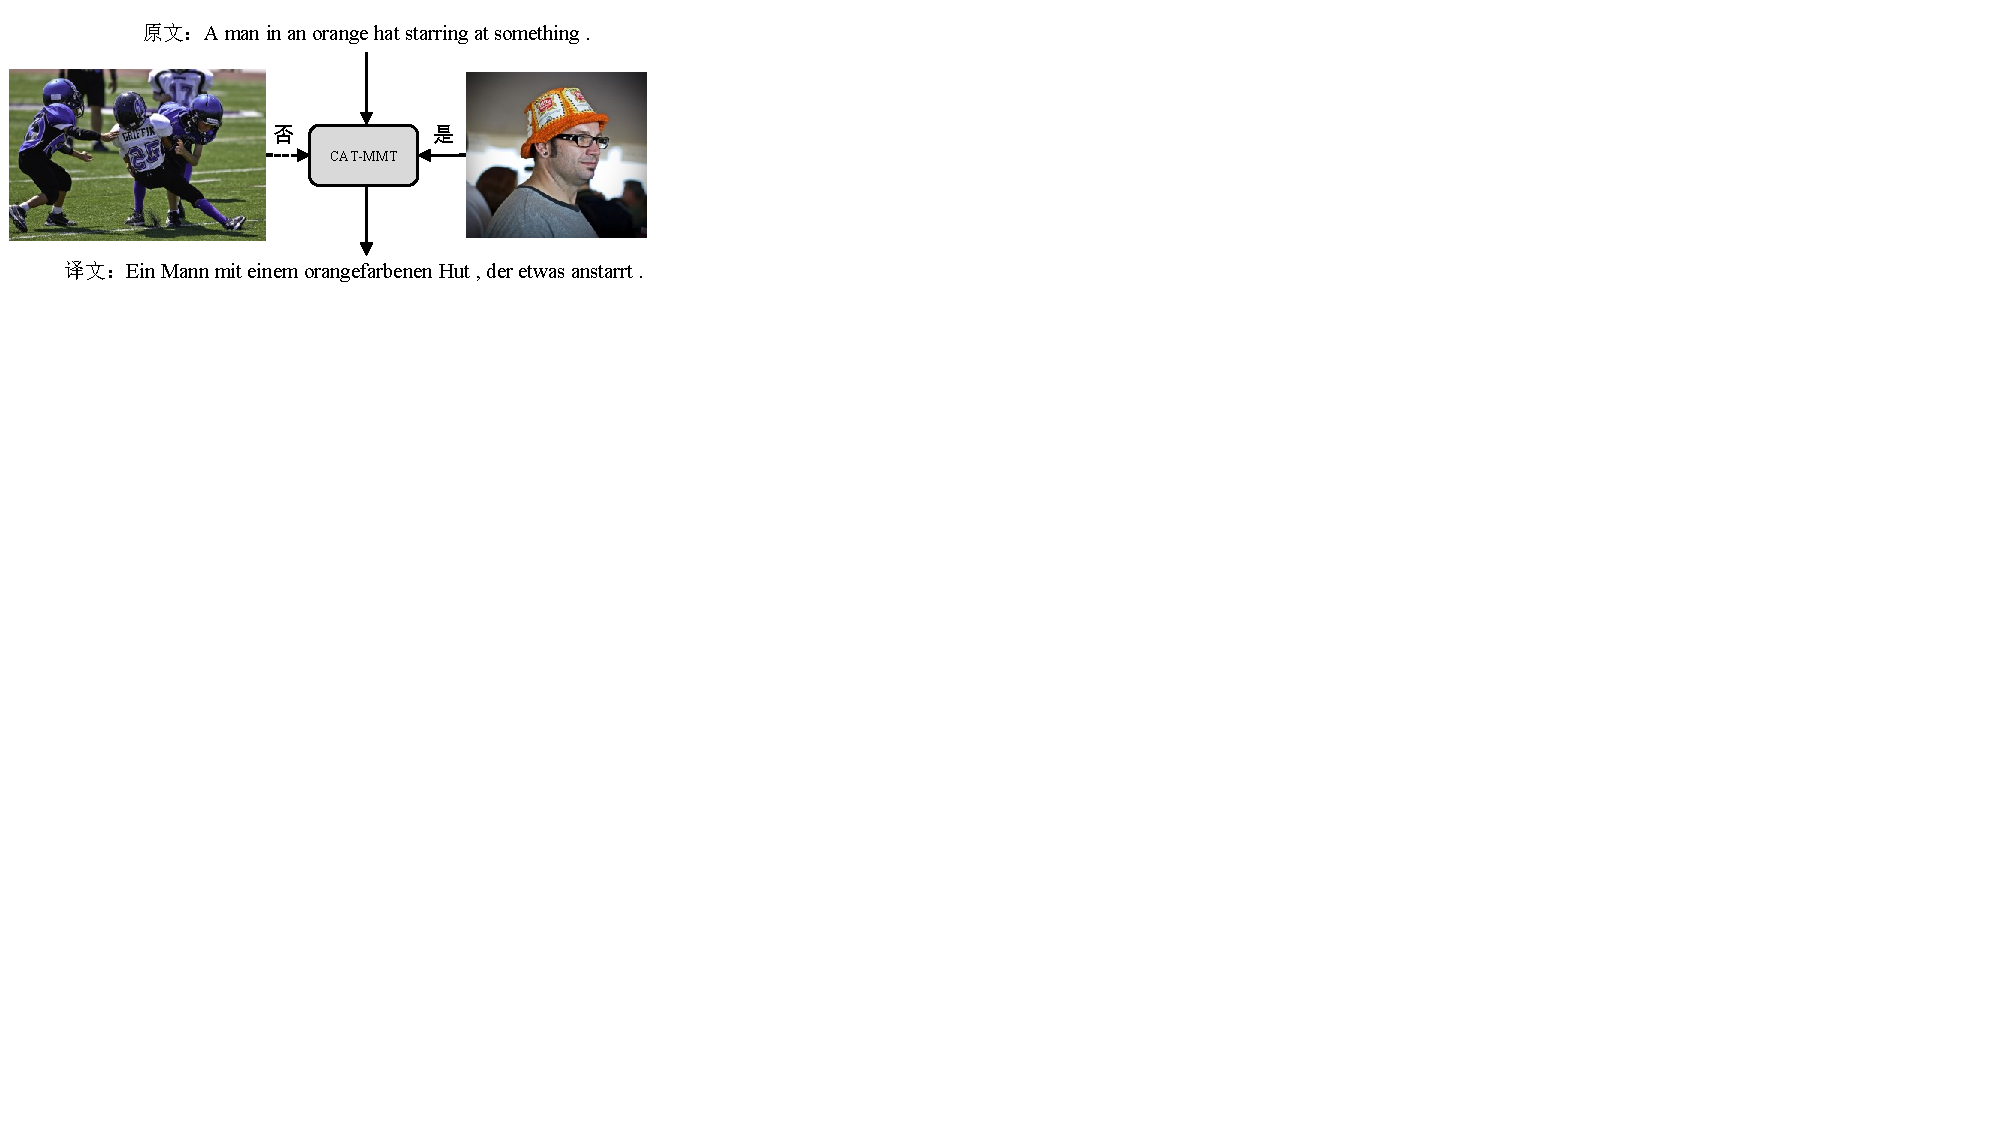
\includegraphics{Img/fig_5_example.pdf}
    \bicaption{引入对抗样本的神经机器翻译模型}{NMT model with adversarial samples}
    \label{fig:5_example}
\end{figure}
已有的相关工作表明在神经机器翻译任务中实现句子级的跨模态语义信息是很困难的。只有少部分的待翻译句子需要额外的输入图片作为信息的补充。大部分的翻译语料已经具备良好的双语对齐关系,这使得融合图片信息的端到端模型在面对更容易学习的并且是文本主导的翻译任务时,并不会过多地关注跨模态的信息对齐与融合。因此,针对神经机器翻译中的句子级跨模态语义融合方法,在讨论图片信息是否以及在哪方面能够为翻译带来质量提升之前,应该更多地关注如何让模型具备从两个模态共同获得信息的能力。为此,本章提出了一种对比对抗训练(contrastive adversarial training, CAT)方法来解决这个问题。首先,我们的模型输入与一般融合图片信息的翻译模型相似,为一个源语言句子和一张对应的图片。其中该图片中的视觉目标被提取出来,并一同输入到模型中。然后我们采用对比学习的方法来拉近输入与译文在统一语义表示空间的距离。其中,译文作为锚点(anchor),将源语言句子与对应的图片作为正样本。为了使模型关注到图片中所携带的视觉信息,我们将源语言句子与随机图片输入到模型中作为负样本。如图\ref{fig:5_example}所示,应用该策略可以强迫翻译模型关注输入的源语言文本与输入图片的语义关系,从而实现句子级别的跨模态信息融合。

%具体贡献
本章主要贡献如下:

% 主要翻译性能上的贡献
(1)本章提出了一种基于图文对比对抗训练的神经机器翻译方法,又称CAT-NMT。在配合双向翻译训练后,对比对抗训练能够有效地为融合图片信息的神经机器翻译方法带来翻译准确率的提升。该方法在三个不同的翻译数据上得到了有效的提升。

% 主要动机上的贡献
(2)本章所提方法旨在将视觉信息融合到本文的表示中,试图通过图片信息加强翻译模型在编码过程中对源语言文本的表示能力,从而提升最终翻译的质量。在对抗实验的分析中可以观察到,CAT-MMT的翻译质量提升来源于成功地将图片信息融合到了文本表示中。因此,CAT方法达到了使翻译模型对视觉信息敏感的目的。

% 分析结果的贡献
(3)在对模型结果的分析中发现,为翻译输入随机图片或不输入图片时,带有歧义词较多的测试集受到的影响最大。该结果可以表明当神经机器翻译模型对视觉信息敏感时,对文本中存在歧义词问题的句子具有更好的翻译效果。
\section{相关工作}
本章工作主要针对将加入对抗样本的对比学习方法应用到融合图片信息的神经机器翻译中,因此相关工作可以分为以下三个部分:

%传统方法:都有哪些方法,这些方法出现的问题,
{\sffamily (1)图片信息辅助式神经机器翻译}
%这里指出简单的方法,和复杂的方法
在融合图片信息的神经机器翻译方法中,将图片作为翻译模型输入的一部分,并将其用于帮助源语言文本的编码或在目标语言生成过程中提供外源参考信息的图片辅助式神经机器翻译是目前最常见的一类。图片可以以多种方式与神经翻译任务相结合,而为了更有效地利用图片信息,研究者们设计了从简单到复杂的图片信息融合方式。文献\cite{52_DBLP:journals/corr/ElliottFH15}将图片的全局特征输入到基于循环神经网络的翻译模型中,将其与源语言句子编码后的隐层向量连接后用于初始化解码器。文献\cite{18_DBLP:conf/emnlp/CalixtoL17}则尝试了更多图片全局特征的使用方法,例如直接初始化编码器,直接初始化解码器以及当做词串接到输入句子的词嵌入后。文献\cite{36_calixto-etal-2017-doubly,47_DBLP:conf/wmt/LibovickyHM18}则利用图片栅格特征可以看作图片特征序列的特性,采用注意力机制为解码器提供动态的上下文信息。这些方法均是通过简单的模型改动达到使神经机器翻译模型支持对视觉特征输入的目的。然而文献\cite{23_elliott-2018-adversarial}的对抗评估则表示以简单的方式将图片输入给模型并不能使图片信息得到很好的利用。在后续的研究进程中涌现了更多复杂的图片信息融合方法。文献\cite{39_ive-etal-2019-distilling}将图片信息作用到解码阶段后的推敲网络(deliberation network)进行二次解码。文献\cite{33_yin-etal-2020-novel}将句子与图片中的视觉目标视为图的关系,采用基于图的编码器融合跨模态信息。
然而文献\cite{53_caglayan-etal-2019-probing}的实验表明,在文本信息缺失的情况下,即便采用简单的图片输入方式,翻译模型也会更多地利用图片信息。因此,对于图片辅助式神经机器翻译方法,需要更多地关注如何使翻译模型更多地关注图片中的信息,从而加强图片信息的辅助作用。

%对比学习方法:主要有NMT的方法,MMT也有相关的概念,但与本文的不同
{\sffamily (2)基于对比学习的神经机器翻译}

对比学习方法已经广泛应用于计算机视觉和自然语言处理的相关研究中。该方法的作用是将样本空间中具有相似语义信息样本点拉近,并增加不相关样本之间的间隙。通常,相似样本之间可互称为正样本,不相关样本之间可互称为负样本。
文献\cite{70_pan-etal-2021-contrastive}在一个多语言神经机器翻译系统中加入了对比学习方法。在训练期间,每个双语翻译对都是正样本,为每对正样本从数据集中随机选取不相关句子作为负样本。在对比损失函数的配合下,针对多语言翻译的交叉熵损失函数能够帮助模型学习到多语言的统一表示空间,从而达到提升多语言之间翻译性能并帮助零资源翻译的目的。
文献\cite{80_li-etal-2021-unimo}提出了一种应用于多模态理解与生成任务的多模态预训练框架。该工作通过对比学习方法建立文本与图片之间的跨模态统一表示空间。在构建过程中,通过计算文本表示与图片表示之间的相似度,实现对来自不同模态信息的语义距离的计算。这种方式能够帮助模型获得更多的跨模态信息,从而更好地服务于下游任务。
文献\cite{37_elliott-kadar-2017-imagination}在训练纯文本的神经机器翻译模型中,引入了“想象力”机制作为翻译的子任务。该机制将文本表示映射到视觉特征的表示空间,尝试通过“想象”的方式使文本表示尽可能地接近图片中的语义。该过程就是利用了对比损失函数,使文本表示尽可能接近对应图片的特征表示,并远离同批数据下其它图片的特征表示。
文献\cite{68_DBLP:journals/corr/KirosSZ14}则是在融合图片信息的神经机器翻译中,通过建立句子与图片统一的表示空间达到应用图片信息提升文本表示的能力的目的,而在构建中同样采用了对比学习的方法。该工作在对比学习中同样加入了对抗样本作为负样本的方式,尝试拉近源语言句子与相关图片在表示空间的距离,并尝试推开与句子不相关的图片,以及推开与图片不相关句子。与该工作不同的是,本章的方法虽然也引入了对抗样本作为负样本,但并不是针对图片与文本之间语义表示的对比学习,而是将图片信息融合到文本的表示中,针对不同文本表示的对比学习,并在该过程中加入了译文作为锚点,使对比学习作用到翻译而不是跨模态表示。

%对抗训练方法:主要用于测试
{\sffamily (3)对抗训练方法}

对抗训练方法常用于在训练神经机器翻译模型时,通过引入对抗样本的方式提升系统的鲁棒性。然而,在融合图片信息的神经机器翻译中,对抗样本更多用于测试输入的图片能否在翻译的过程中起作用。
文献\cite{23_elliott-2018-adversarial}提出采用对抗评估来测试翻译模型是否利用到视觉信息。该研究在融合图片信息的神经机器翻译模型中输入与文本相对应和不对应的图片,然后通过测试模型的翻译准确率的变化来判断模型在翻译过程中是否受到输入图片信息的影响。
文献\cite{20_wu-etal-2021-good,22_li-etal-2021-vision}在分析视觉信息是否在翻译模型中起作用时,同样使用了对抗样本的方法。该工作认为图片与噪音的作用相似,是通过正则化(regularization)的方式提升了翻译模型的性能。
文献\cite{23_elliott-2018-adversarial}则采用了文本对抗输入的方式测试融合图片信息的神经机器翻译模型能否通过图片中的信息纠正对抗文本带来的错误。其结果表明图片信息无法做到纠正文本错误。这一结果也说明了虽然模型的输入同时包含了来自图片和文本两个模态的信息,但融合图片信息的神经机器翻译仍然是文本信息为主图片信息为辅的。
与以上工作在测试阶段应用对抗样本不同的是,本章所提方法将对抗样本应用于对比学习的训练过程。对抗样本作为负样本能够在对比学习的语义聚类过程中,帮助模型结合更细粒度的语义信息,从而使模型能够分辨出输入的图片信息是否与文本内容一致。
\section{方法描述}
\label{sec:5_method}

对于一个标准的图片信息辅助式神经机器翻译,其输入为一个源语言句子$X$和一个与其对应的图片$I$,然后利用这两个模态的信息生成翻译$Y$。然而,现有的很多方法对输入图片$I$中的信息并不敏感。这是因为翻译任务所使用的语料中,大部分$X$与$Y$之间有着很好的语义对齐关系。这使得翻译模型在不依靠图片输入的情况下,就可以在训练阶段学习到一组相对不错的模型参数,使模型很容易收敛到一个不需要图片信息的局部最优解。为了使模型充分利用为待翻译句子所提供的视觉信息,本章提出了基于图文对比对抗训练的神经机器翻译方法。本节将首先介绍本章所使用的翻译模型结构,然后详细介绍如何通过对比对抗训练增加模型对视觉信息的敏感度。

\subsection{模型结构}
\label{sec:5_architecture}
本章采用了一种句子级跨模态语义融合模型结构,其输入为一个文本序列,和一个可选的视觉输入,该视觉输入为文本序列所对应的完整图片以及图片内部的数个视觉目标,如图【】所示。该模型的编码器和解码器为一般的Transformer结构。其中,Transformer的编码器负责跨模态信息融合。为了使Transformer支持文本加图片形式的输入,我们采用了一个多模态嵌入层。该嵌入层共分为4个子层:词嵌入层,视觉特征层,模态分割层,位置编码层。

(1){\sffamily 词嵌入层:}为了支持图片的输入,需要在词嵌入层所对应的词表中,加入一些特殊字符:“<seg>”将词嵌入层输入的前后两部分分割为文本和视觉两个序列;“<img>”代表着放置完整图片的位置,每个输入序列仅一个;“<bbx>”代表放置图片中的视觉目标的位置,每个输入序列可以有多个;“<end>”代表着多模态输入序列的结尾。


(2){\sffamily 视觉特征层:}该层每个位置的输入与词嵌入层的特殊字符相对应,其中“<img>”的对应位置放置输入的完整图片的全局特征,“<bbx>”对应位置放置视觉目标的图片全局特征,其它位置则输入零向量。


(3){\sffamily 分割层:}这一层的作用相对简单,主要用作标识每个位置的输入属于文本序列还是图片序列。因此一共只有“文本模态”和“视觉模态”两个值,每个在模型中是一个与词嵌入层维度相同的向量。其中“<seg>”之前的文本序列均对应着“文本模态”,“<seg>”以及其后面的序列均为“视觉模态”。


(4){\sffamily 位置向量层:}这一层与一般的位置向量作用相似,能够表示输入序列中的绝对位置关系。区别在于,当输入的视觉目标与文本中的某些词有对应关系时,可以将视觉目标的位置设置为与其对应的词相同的位置,从而达到加强图片信息作用准确性的目的。如图【】所示,图片输入序列中的“帽子”的绝对位置为5,与文本序列中的“hat”保持一致。

在解码阶段,解码器仅接收“文本模态”的编码结果作为输入。这是因为本章的CAT方法旨在帮助神经机器翻译模型将视觉信息融合到文本表示中。而该过程发生在编码阶段,即没有针对解码器采取翻译以外的优化方法。因此,基于一般的翻译模型对视觉信息不敏感的假设,其内部模块,如解码器,往往也会忽略视觉信息的输入。所以,将“视觉模态”部分的隐层单元传递给解码器是多余的。

图【】中可以看到,CAT-MMT的目标函数包含了两个部分:融合图片信息的神经机器翻译所需的交叉熵损失函数和CAT所需的对比损失函数。其中交叉熵损失函数为:
\begin{equation}
    L_{CE}(\phi, \theta, \psi)=-\sum_j^M \log p(y_j|y_{<j},X,I)
\label{eq:5_cross_entropy}
\end{equation}
其中,$y_j \in Y,j=1,\cdots,M$,$\phi$为解码器参数,$\theta$为编码器参数,$\psi$为多模态嵌入层的参数。该损失函数与一般的融合图片信息的神经机器翻译模型的相似,均是通过源语言文本$X$和对应图片$I$为输入信息,生成翻译$Y$的形式。在我们的方案中,$I$代表了完整的图片与其中的多个视觉目标的组合。该损失函数无法反映出的信息是,本章的跨模态信息融合过程,仅发生在编码端。图【】中除了平均池化(average pooling)层,其它参数均需要通过翻译任务来优化。

\subsection{对比对抗训练}
\label{sec:5_cat}
正如\ref{sec:5_architecture}小节所介绍,本章是在Transformer的编码器中实现将跨模态信息融合到文本的表示中。然而,基于一般的翻译模型对视觉信息不敏感的假设,在没有额外的引导下,编码器同样会忽略图片信息的存在。为了有效地融合视觉信息,本章提出了图文对比对抗方法来实现在编码过程将图片中的视觉信息融合到文本的表示中。CAT方法主要包含三部分:对比学习,对抗样本以及双向翻译训练。

{\sffamily 对比学习}

对比学习方法能够在语义表示空间中拉近相似的样本,推离不相关的样本。针对融合图片信息神经翻译中,将目标译文$Y$作为锚点,将编码端的输入$X+I$作为正样本。在$X$与$Y$的双语统一表示空间中,对比学习方法能够拉近$X+I$与$Y$之间的距离,并将其它的所有样本视为负样本,拉开与$X+I$和$Y$之间的距离。图【】中每个圆代表文本语义表示空间的一个点,其中图【】(a)和图【】(b)展示了对比学习将表示空间的样本分簇归类的能力,图【】(b)中的每个簇可视为一个双语平行句对。常规的对比学习损失函数为:
\begin{equation}
    \mathcal{L}_{CL}(\theta, \psi)=-\log\ \frac{e^{\mathrm{sim}(\mathcal{R}(Y),\mathcal{R}(X+V))/\tau}}{\sum_{Z\in N}e^{\mathrm{sim}(\mathcal{R}(Y),\mathcal{R}(Z))/\tau}}
    \label{eq:5_contrastive_learning}
\end{equation}

其中$\mathrm{sim}(\cdot,\cdot)$为余弦相似度函数,用于计算两个表示向量的语义相似度;$\tau$为温度,控制区分正负样本的能力;$\mathcal{R}(\cdot)$代表平均池化,正如图【】所示,对比损失的输入是文本表示经平均池化后的结果;$N$代表着负样本集。

$\mathcal{L}_{CL}$与$\mathcal{L}_{CE}$之间共享编码器和嵌入层的参数,因此本章所采用的对比学习只针对编码器进行参数优化。


\section{实验设置}

\section{实验结果}

\section{本章小结}
